\section{Echo State Networks}
Echo State Networks, seyrek bağlantılı bir gizli katmana ve sabit ağırlıklara sahiptir. Zaman serisi verilerini işlemek için kullanılır. 

\begin{figure}[h]
    \centering
    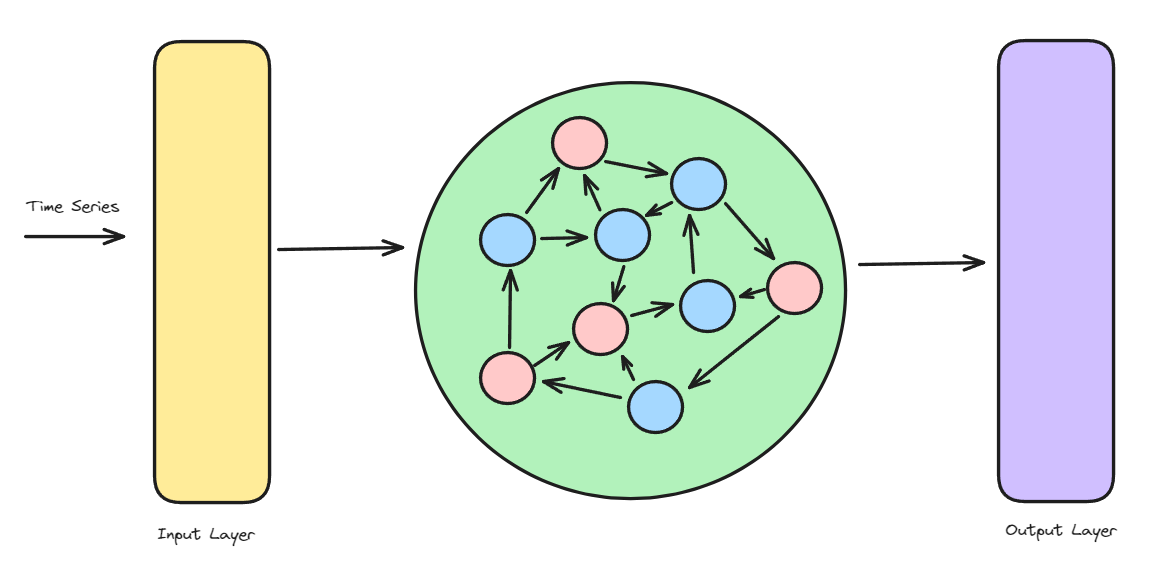
\includegraphics[width=1\textwidth]{images/echo_state_network.png}
    \caption{Yankı durumu makinesi mimarisi.}
    \label{fig:enter-label}
\end{figure}

\subsection{Çalışma Adımları}
\begin{enumerate}
    \item Bağlantıları rastgele atanmış, LSM ile benzerlik gösteren Rezervuar adı verilen ağ oluşturulur.
    \item Giriş verisi rezervuar içindeki nöronlarla etkileşime girer. Bu etkileşimler, zamanla değişen dinamik bir durumu temsil eden bir uç durum oluşturur.
    \item Bu iç durum çıkış katmanına iletilir. ESN, çıkış katmanındaki parametrelerin ayarlanmasıyla eğitilir.
\end{enumerate}

\newpage